\documentclass{standalone}
\usepackage{pgfplots}
\pgfplotsset{compat=1.17}

\begin{document}
\begin{tikzpicture}

% ----------------------------------------------------------
%   MAIN SCATTER PLOT  (x-axis: system ↔ user  –  y: complexity)
% ----------------------------------------------------------
\begin{axis}[
        width=24cm,
        height=12cm,
        xmin=0, xmax=10,
        ymin=0, ymax=10,
        xlabel={System-centric \hspace{16.5cm} User-centric},
        ylabel={Complexity},
        xtick=\empty,
        ytick=\empty,
        axis lines=left,
        grid=major,
        grid style={gray!25},
        nodes near coords,
        every axis plot/.append style={very thick, opacity=0.3},
        nodes near coords style={black,font=\small,text width=4cm,align=center,opacity=0.3},
    ]

% ========== CONVERSATIONAL  (▲)  ==========
\addplot[only marks,
         mark=triangle*,
         mark size=4pt,
         mark options={fill=red,draw=red},
         point meta=explicit symbolic] coordinates{
  (6, 7)   [\textbf{SimIIR-3}\\(Azzopardi et al., 2024)]
  (6.5, 8)   [\textbf{CSHI}\\(Zhu et al., 2024)]
  (5, 8)   [\textbf{ConvLab-2}\\(Lee et al., 2019)]
  (5.5, 6)   [\textbf{ConvLab-3}\\(Zhu et al., 2023)]
  (8.9, 5.2) [\textbf{UserSimCRS}\\(Afzali et al., 2023)]
  (7.4, 4) [\textbf{PyDial}\\(Ultes et al., 2017)]
  (8.4, 2.8) [\textbf{SimDial}\\(Zhao et al., 2018)]
  (9, 1.2) [\textbf{CBL}\\(Thies et al., 2022)]
  (4.9, 5.2) [\textbf{SimLab}\\(Bernard et al., 2025)]
  (8, 7.4) [\textbf{RecUserSim}\\(Chen et al., 2025)]
  (8.7, 4.1) [\textbf{GenIRSim}\\(Kiesel et al., 2024)]
};

% -------- CONVERSATIONAL – Evaluation (▲, blue) --------
\addplot[only marks,
         mark=triangle*,
         mark size=4pt,
         mark options={fill=blue,draw=blue},
         point meta=explicit symbolic] coordinates{
  (8.1, 6) [\textbf{iEvaLM}\\(Wang et al., 2023)]
};

% ========== SEARCH  (◆) –- Simulation ==========
\addplot[only marks,
         mark=diamond*,
         mark size=4pt,
         mark options={fill=red,draw=red},
         point meta=explicit symbolic] coordinates{
  (8, 8.5)   [\textbf{BASES}\\(Ren et al., 2024)]
  (9.1, 6.4)   [\textbf{USimAgent}\\(Zhang et al., 2024)]
  (6.8, 6.2)   [\textbf{SimIIR2.0}\\(Zerhoudi et al., 2022)]
  (7.2, 5.1) [\textbf{SimIIR}\\(Maxwell et al., 2016)]
  (6.8, 3.2) [\textbf{PyClick}\\(Chuklin et al., 2015)]
};

% -------- SEARCH – Hybrid (◆, green) -----------
\addplot[only marks,
         mark=diamond*,
         mark size=4pt,
         mark options={fill=green,draw=green},
         point meta=explicit symbolic] coordinates{
  (2, 8.6)   [\textbf{UBS4RL}\\(Zhang et al., 2022)]
};

% -------- SEARCH – Evaluation (◆, blue) --------
\addplot[only marks,
         mark=diamond*,
         mark size=4pt,
         mark options={fill=blue,draw=blue},
         point meta=explicit symbolic] coordinates{
  (1.5, 7)   [\textbf{CloudSim-Search}\\(Bendechache et al., 2019)]
  (2, 3.2) [\textbf{Expected Global Utility}\\(Yang \& Lad, 2009)]
  (4, 3.2) [\textbf{CoSearcher}\\(Salle et al., 2022)]
  (0.8, 1.5) [\textbf{cwl\_eval}\\(Azzopardi et al., 2019)]
};

% -------- SEARCH – Other (◆, orange) -----------
\addplot[only marks,
         mark=diamond*,
         mark size=4pt,
         mark options={fill=orange,draw=orange},
         point meta=explicit symbolic] coordinates{
  (6, 2.2) [\textbf{ClickChainSim}\\(Chuklin et al., 2016)]
};

% ========== RECOMMENDER  (■) – Simulation =======
\addplot[only marks,
         mark=square*,
         mark size=3pt,
         mark options={fill=red,draw=red},
         point meta=explicit symbolic] coordinates{
  (3.7, 9)   [\textbf{Virtual-Taobao}\\(Shi et al., 2018)]
  (3.3, 8)   [\textbf{RecSimNG}\\(Mladenov et al., 2021)]
  (3, 7)   [\textbf{KuaiSim}\\(Zhao et al., 2023)]
  (2.8, 6)   [\textbf{RecSim}\\(Ie et al., 2019)]
  (2.3, 5)   [\textbf{Sim4Rec}\\(Sberbank, 2022)]
  (2, 2)   [\textbf{RecoGym}\\(Rohde et al., 2018)]
  (9.4, 3.3)   [\textbf{Lusifer}\\(Ebrat et al., 2025)]
  (6, 4.5)   [\textbf{SUBER}\\(Corecco et al., 2024)]
};

% -------- RECOMMENDER – Evaluation (■, blue) ----
\addplot[only marks,
         mark=square*,
         mark size=3pt,
         mark options={fill=blue,draw=blue},
         point meta=explicit symbolic] coordinates{
  (7.9, 2) [\textbf{SIREN}\\(Bountouridis et al., 2019)]
  (2.6, 1.2) [\textbf{LensKit}\\(Hug et al., 2020)]
};

% -------- RECOMMENDER – Hybrid (■, green) -------
\addplot[only marks,
         mark=square*,
         mark size=3pt,
         mark options={fill=green,draw=green},
         point meta=explicit symbolic] coordinates{
  (6, 1)   [\textbf{T-RECS}\\(Lucherini et al., 2021)]
};

% ----------------------------------------------------------
%   HIGHLIGHTED FRAMEWORKS (opacity = 1)
% ----------------------------------------------------------

% --- Conversational – Simulation (▲ red, opacity 1) ---
\addplot[only marks,
         mark=triangle*,
         mark size=4pt,
         mark options={fill=red,draw=red,opacity=1},
         nodes near coords,
         nodes near coords style={black,font=\small,text width=4cm,align=center,opacity=1},
         point meta=explicit symbolic] coordinates{
  (6, 7)   [\textbf{SimIIR-3}\\(Azzopardi et al., 2024)]
  (5.5, 6) [\textbf{ConvLab-3}\\(Zhu et al., 2023)]
  (7.4, 4) [\textbf{PyDial}\\(Ultes et al., 2017)]
  (8.9, 5.2) [\textbf{UserSimCRS}\\(Afzali et al., 2023)]
  (8.7, 4.1) [\textbf{GenIRSim}\\(Kiesel et al., 2024)]
};

% --- Conversational – Evaluation (▲ blue, opacity 1) --- 
\addplot[only marks,
         mark=triangle*,
         mark size=4pt,
         mark options={fill=blue,draw=blue,opacity=1},
         nodes near coords,
         nodes near coords style={black,font=\small,text width=4cm,align=center,opacity=1},
         point meta=explicit symbolic] coordinates{
  (8.1, 6) [\textbf{iEvaLM}\\(Wang et al., 2023)]
};

% --- Search – Simulation (◆ red, opacity 1) ---
\addplot[only marks,
         mark=diamond*,
         mark size=4pt,
         mark options={fill=red,draw=red,opacity=1},
         nodes near coords,
         nodes near coords style={black,font=\small,text width=4cm,align=center,opacity=1},
         point meta=explicit symbolic] coordinates{
  (7.2, 5.1) [\textbf{SimIIR}\\(Maxwell et al., 2016)]
  (6.8, 6.2) [\textbf{SimIIR2.0}\\(Zerhoudi et al., 2022)]
};

% --- Search – Evaluation (◆ blue, opacity 1) ---
\addplot[only marks,
         mark=diamond*,
         mark size=4pt,
         mark options={fill=blue,draw=blue,opacity=1},
         nodes near coords,
         nodes near coords style={black,font=\small,text width=4cm,align=center,opacity=1},
         point meta=explicit symbolic] coordinates{
  (0.8, 1.5) [\textbf{cwl\_eval}\\(Azzopardi et al., 2019)]
  (4, 3.2) [\textbf{CoSearcher}\\(Salle et al., 2022)]
};

% --- Recommender – Simulation (■ red, opacity 1) ---
\addplot[only marks,
         mark=square*,
         mark size=3pt,
         mark options={fill=red,draw=red,opacity=1},
         nodes near coords,
         nodes near coords style={black,font=\small,text width=4cm,align=center,opacity=1},
         point meta=explicit symbolic] coordinates{
  (2.8, 6)   [\textbf{RecSim}\\(Ie et al., 2019)]
  (3.3, 8)   [\textbf{RecSimNG}\\(Mladenov et al., 2021)]
  (2.3, 5)   [\textbf{Sim4Rec}\\(Sberbank, 2022)]
  (3, 7)   [\textbf{KuaiSim}\\(Zhao et al., 2023)]
  (9.4, 3.3)   [\textbf{Lusifer}\\(Ebrat et al., 2025)]
};

% --- Recommender – Evaluation (■ blue, opacity 1) ---
%\addplot[only marks,
%         mark=square*,
%         mark size=3pt,
%         mark options={fill=blue,draw=blue,opacity=1},
%         nodes near coords,
%         nodes near coords style={black,font=\small,text width=4cm,align=center,opacity=1},
%         point meta=explicit symbolic] coordinates{
%  (2.6, 1.2) [\textbf{LensKit}\\(Hug et al., 2020)]
%};

\end{axis}

% ----------------------------------------------------------
%   COMPACT TOP-LEGENDS (Category  |  Type)
% ----------------------------------------------------------

% Category legend (left side)
\node[anchor=south west, text opacity=1, rounded corners=0pt, inner sep=3pt]
      at (rel axis cs:0.005,1.02) {%%
  \begin{tikzpicture}[baseline]
    \node[font=\footnotesize\bfseries] at (0, -0.05) {Category:};
    \node at (1.8,0) {\tikz\draw[fill=black] (0,0) -- ++(0.16,0.28) -- ++(-0.32,0) -- cycle;};
    \node[font=\footnotesize] at (2.3,0) {Conversational};
    \node at (4.8,0) {\tikz\draw[fill=black] (0,0) rectangle (0.25,0.25);};
    \node[font=\footnotesize] at (5.2,0) {Recommender};
    \node at (7.6,0) {\tikz\draw[fill=black] (0.15,0) -- ++(0.15,0.15) -- ++(-0.15,0.15) -- ++(-0.15,-0.15) -- cycle;};
    \node[font=\footnotesize] at (8.1,0) {Search};
  \end{tikzpicture}}
;

% Framework-type legend (right side)
\node[anchor=south east, text opacity=1, rounded corners=0pt, inner sep=3pt]
      at (rel axis cs:0.995,1.02) {%%
  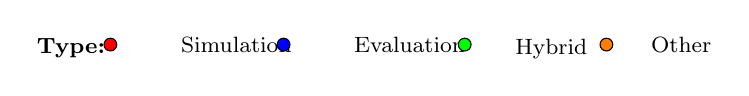
\begin{tikzpicture}[baseline]
    \node[font=\footnotesize\bfseries] at (-0.6, -0.05) {Type:};
    \node at (-0.1,0) {\tikz\draw[fill=red] (0,0) circle (2.3pt);};
    \node[font=\footnotesize] at (1.5,0) {Simulation};
    \node at (2.1,0) {\tikz\draw[fill=blue] (0,0) circle (2.3pt);};
    \node[font=\footnotesize] at (3.7,0) {Evaluation};
    \node at (4.4,0) {\tikz\draw[fill=green] (0,0) circle (2.3pt);};
    \node[font=\footnotesize] at (5.5, -0.05) {Hybrid};
    \node at (6.2,0) {\tikz\draw[fill=orange] (0,0) circle (2.3pt);};
    \node[font=\footnotesize] at (7.15, 0) {Other};
  \end{tikzpicture}}
;

\end{tikzpicture}
\end{document}
